\documentclass[unicode,11pt,a4paper,oneside,numbers=endperiod,openany]{scrartcl}

\usepackage{graphicx}
\usepackage{float}
\usepackage{subcaption}

\input{assignment.sty}
\graphicspath{./img/}

\def\imgHeightHelicopter{7cm}
\def\imgHeightSkirt{12cm}
\def\imgHeightde2010{11cm}

\begin{document}


\setassignment
\setduedate{Wednesday, 25 October 2023, 11:59 PM}

\serieheader{Numerical Computing}
{2023}
{Student: Jeferson Morales Mariciano \\}
{Discussed with: Michele Dalle Rive, Martin Lettry}
{Solution for Project 2}{}
\newline

\assignmentpolicy

\newpage

%%%%%%%%%%%%%%%%%%%%%%%%%%%%%%%%%%%%%%%%%%%%%%%%%%
\section{The assignment}
%%%%%%%%%%%%%%%%%%%%%%%%%%%%%%%%%%%%%%%%%%%%%%%%%%

Tests environment:
\begin{itemize}
    \item Ubuntu 22.04.1
    \item Linux kernel 6.2.0-35 generic
    \item Matlab R2023b
    \item Metis version provided
\end{itemize}

\subsection{Implement various graph partitioning algorithms [50 points]}

The results are obtained by running `Bench\_bisection.m` after implementing spectral and inertial methods in
correspondent `bisection\_spectral.m` and `bisection\_inertial.m` files.

For spectral implementaion, the threshold has been choosen to be $0$, since it reports better results generally for our meshesh. \\

\begin{table}[H]
    \caption{Bisection results, cutsizes for each method}
    \centering
    \begin{tabular}{l|r|r|r|r} \hline\hline
        Mesh                       & Coordinate & Metis 5.0.2 & Spectral & Inertial \\ \hline
        grid5rec(12,100)           & 12         & 12          & 12       & 12       \\
        grid5rec(100,12)           & 12         & 12          & 12       & 12       \\
        grid5recRotate(100,12,-45) & 22         & 12          & 12       & 12       \\
        gridt(50)                  & 72         & 82          & 70       & 72       \\
        grid9(40)                  & 118        & 127         & 128      & 118      \\
        Smallmesh                  & 25         & 12          & 12       & 30       \\
        Tapir                      & 55         & 23          & 18       & 49       \\
        Eppstein                   & 42         & 41          & 42       & 45       \\
        \hline \hline
    \end{tabular}
    \label{table:bisection}
\end{table}

\begin{table}[H]
    \caption{Bisection timings for each method, matlab `timeit()` function}
    \centering
    \begin{tabular}{l|r|r|r|r} \hline\hline
        Mesh                       & Coordinate & Metis 5.0.2 & Spectral & Inertial   \\ \hline
        grid5rec(12,100)           & 0.0015     & 0.0013      & 0.024    & 3.0764e-04 \\
        grid5rec(100,12)           & 0.0014     & 0.0017      & 0.0261   & 3.1754e-04 \\
        grid5recRotate(100,12,-45) & 0.0019     & 0.0017      & 0.0256   & 3.1954e-04 \\
        gridt(50)                  & 0.0020     & 0.0019      & 0.0537   & 3.9554e-04 \\
        grid9(40)                  & 0.0019     & 0.0028      & 0.0635   & 3.5784e-04 \\
        Smallmesh                  & 3.1284e-04 & 3.3817e-04  & 0.0084   & 2.5849e-04 \\
        Tapir                      & 0.0020     & 0.0020      & 0.0300   & 3.2250e-04 \\
        Eppstein                   & 0.0012     & 0.0017      & 0.0200   & 3.3750e-04 \\
        \hline \hline
    \end{tabular}
    \label{table:bisection-timings}
\end{table}

With the provided Table \ref{table:bisection} it's evident that all methods produce identical results for some test cases
(e.g., grid5rec(12,100), grid5rec(100,12), and others), reinforcing the idea that Coordinate, Metis, and
Spectral may not significantly differ in these specific scenarios.
Nevertheless, it's essential to consider the computational costs and accuracy trade-offs when choosing a graph partitioning methodology,
as accuracy and performance can vary substantially across different cases. \\

Confronting with Table \ref{table:bisection-timings} timings, it has been observed that Inertial is the quickest of the methods
even though the one producing most edgecuts generally, hence worse quality paritioning.
Spectral method is the one with fewest edgecuts and also the method taking the longest time to compute the partitioning
since its computational task is to calculate eigenvectors and eigenvalues for large mesh matrices.
Coordinate and Metis in terms of timing are generally similar in timing and edgecuts, with Metis being slightly slower and producing more edgecuts. \\
\cleardoublepage

\subsection{Recursively bisecting meshes [20 points]}

The results are obtained by running `Bench\_rec\_bisection.m`. \\

\begin{table}[H]
    \caption{Edge-cut results for recursive bi-partitioning with $p=8$.}
    \centering
    \begin{tabular}{l|r|r|r|r} \hline\hline
        Case      & Spectral & Metis 5.0.2 & Coordinate & Inertial \\ \hline
        mesh3e1   & 51       & 57          & 63         & 59       \\
        bodyy4    & 1000     & 985         & 1065       & 1364     \\
        de-2010   & 809      & 491         & 929        & 1084     \\
        biplane-9 & 411      & 465         & 548        & 648      \\
        L-9       & 718      & 637         & 631        & 828      \\  \hline \hline
    \end{tabular}
    \label{table:rec_p8}
\end{table}

\begin{table}[H]
    \caption{Edge-cut results for recursive bi-partitioning with $p=16$.}
    \centering
    \begin{tabular}{l|r|r|r|r} \hline\hline
        Case      & Spectral & Metis 5.0.2 & Coordinate & Inertial \\ \hline
        mesh3e1   & 61       & 57          & 63         & 59       \\
        bodyy4    & 1675     & 1591        & 1951       & 2214     \\
        de-2010   & 1512     & 897         & 1796       & 2002     \\
        biplane-9 & 794      & 845         & 974        & 1093     \\
        L-9       & 1121     & 1019        & 1028       & 1377     \\  \hline \hline
    \end{tabular}
    \label{table:rec_p16}
\end{table}

By applying recursive partitioning algorithms, the graph is repeatedly divided into two additional subgraphs every time.
Such approach has a clear advantage when aiming to parallelize and scale the computation of partitions and then the workload
in a distributed system. \\

The number of subgraphs into which the graphs is splitted is $2^{levels}$, where $levels$ represents the number of recursion levels.
It's important to notice that the partitions generated at each recursion level have a fundamental impact on all subsequent recursions.
As an example, small imbalances in partitions would get amplified at each recursion level. \\

During benchmarking, from tables \ref{table:rec_p8}, \ref{table:rec_p16} it becomes evident that the spectral method suffers of performance degradation when transitioning  to larger graphs and computing eigenvectors and eigenvalues.
Even Metis and Coordinate suffers from such transition to larger graph, but the magnitude of the issue changes with respect to the case.
Inertial method always show to have the most edgecuts, indicating lower performance, and it worse as the number
of partitions increases.
Coordinate show to be around the meadian of the number of edgecuts of all the other methods, since generally
performing worse than spectral and metis, but not as magnitudinally worse as inertial. \\

Visualization for case \textit{"de-2010"} is provided for $p=8$ and $p=16$ in Figure \ref{fig:de2010-rec-kway-8} and
\ref{fig:de2010-rec-kway-16} respectively.

\begin{figure}[H]
    \begin{minipage}[H]{.45\textwidth}
        \centering
        \includegraphics[height=\imgHeightde2010, width=1\textwidth, trim={0 0.5cm 0 0}, clip]{./img/ex2/de2010-coord-8.eps}
        \subcaption{Coordinate, $929$ edgecuts}\label{fig:de2010-coord-8}
    \end{minipage}
    \hfill
    \begin{minipage}[H]{.45\textwidth}
        \centering
        \includegraphics[height=\imgHeightde2010, width=1\textwidth, trim={0 0.5cm 0 0}, clip]{./img/ex2/de2010-met-8.eps}
        \subcaption{Metis, $491$ edgecuts}\label{fig:de2010-metis-8}
    \end{minipage}
    \newline
    \begin{minipage}[H]{.45\textwidth}
        \centering
        \includegraphics[height=\imgHeightde2010, width=1\textwidth, trim={0 0.5cm 0 0}, clip]{./img/ex2/de2010-spect-8.eps}
        \subcaption{Recursive bisection, $809$ edgecuts}\label{fig:de2010-spec-8}
    \end{minipage}
    \hfill
    \begin{minipage}[H]{.45\textwidth}
        \centering
        \includegraphics[height=\imgHeightde2010, width=1\textwidth, trim={0 0.5cm 0 0}, clip]{./img/ex2/de2010-inert-8.eps}
        \subcaption{K-way direct partitioning, $1084$ edgecuts}\label{fig:de2010-inert-8}
    \end{minipage}
    \caption{\textit{de-2010} mesh - method confront with $8$ partitions}
    \label{fig:de2010-rec-kway-8}
\end{figure}


\begin{figure}[H]
    \begin{minipage}[H]{.45\textwidth}
        \centering
        \includegraphics[height=\imgHeightde2010, width=1\textwidth, trim={0 0.5cm 0 0}, clip]{./img/ex2/de2010-coord-16.eps}
        \subcaption{Coordinate, $1796$ edgecuts}\label{fig:de2010-coord-16}
    \end{minipage}
    \hfill
    \begin{minipage}[H]{.45\textwidth}
        \centering
        \includegraphics[height=\imgHeightde2010, width=1\textwidth, trim={0 0.5cm 0 0}, clip]{./img/ex2/de2010-met-16.eps}
        \subcaption{Metis, $897$ edgecuts}\label{fig:de2010-metis-16}
    \end{minipage}
    \newline
    \begin{minipage}[H]{.45\textwidth}
        \centering
        \includegraphics[height=\imgHeightde2010, width=1\textwidth, trim={0 0.5cm 0 0}, clip]{./img/ex2/de2010-spect-16.eps}
        \subcaption{Recursive bisection, $1512$ edgecuts}\label{fig:de2010-spec-16}
    \end{minipage}
    \hfill
    \begin{minipage}[H]{.45\textwidth}
        \centering
        \includegraphics[height=\imgHeightde2010, width=1\textwidth, trim={0 0.5cm 0 0}, clip]{./img/ex2/de2010-inert-16.eps}
        \subcaption{K-way direct partitioning, $2002$ edgecuts}\label{fig:de2010-inert-16}
    \end{minipage}
    \caption{\textit{de-2010} mesh - method confront with $16$ partitions}
    \label{fig:de2010-rec-kway-16}
\end{figure}
\cleardoublepage

\subsection{Comparing recursive bisection to direct k-way partitioning [15 points]}

The results are obtained by running `Bench\_metis.m`.

\begin{table}[H]
    \caption{Comparing edge cuts number for recursive bisection and direct multiway partitioning in Metis 5.0.2.}
    \centering
    \begin{tabular}{l|r|r} \hline\hline
        Partitions                & Helicopter & Skirt \\ \hline
        16 - recursive bisection  & 343        & 3119  \\
        16 - way direct partition & 324        & 3393  \\
        32 - recursive bisection  & 537        & 6075  \\
        32 - way direct partition & 539        & 6051  \\  \hline \hline
    \end{tabular}
    \label{table:compare_metis}
\end{table}

By looking at the data, we immediately see that the switch from $16$ to $32$ of the same graph almost
double the amount of cut edges, regardless of the graph partitioning method used. \\

From table \ref{table:compare_metis} we can see that neither recursive nor bisection method is better
than the other:
although there are cases where one method is better than the other, the overall total results show evenly distributed
best result for both methods.\\

Recursive bisection is performing worst for Helicopter with $16$ partitions, but notice that is
performing best for skirt of the same number of partitions.
Then, you would assume recursive is best for skirt and worst for helicopter, but for $32$ partitions the results are inverted:
recursive is best for helicopter and worst for skirt.\\

Figures of helicopter and skirt with $32$ partitions are visualized for both methods using `rotate3d` Matlab figure property. \\

\begin{figure}[H]
    \begin{minipage}[H]{.45\textwidth}
        \centering
        \includegraphics[width=1\textwidth, trim={0 0.5cm 0 0.4cm}, clip]{./img/ex3/heli-rec-front-32}
        \subcaption{Recursive bisection front view}\label{fig:heli-rec-front-32}
    \end{minipage}
    \hfill
    \begin{minipage}[H]{.45\textwidth}
        \centering
        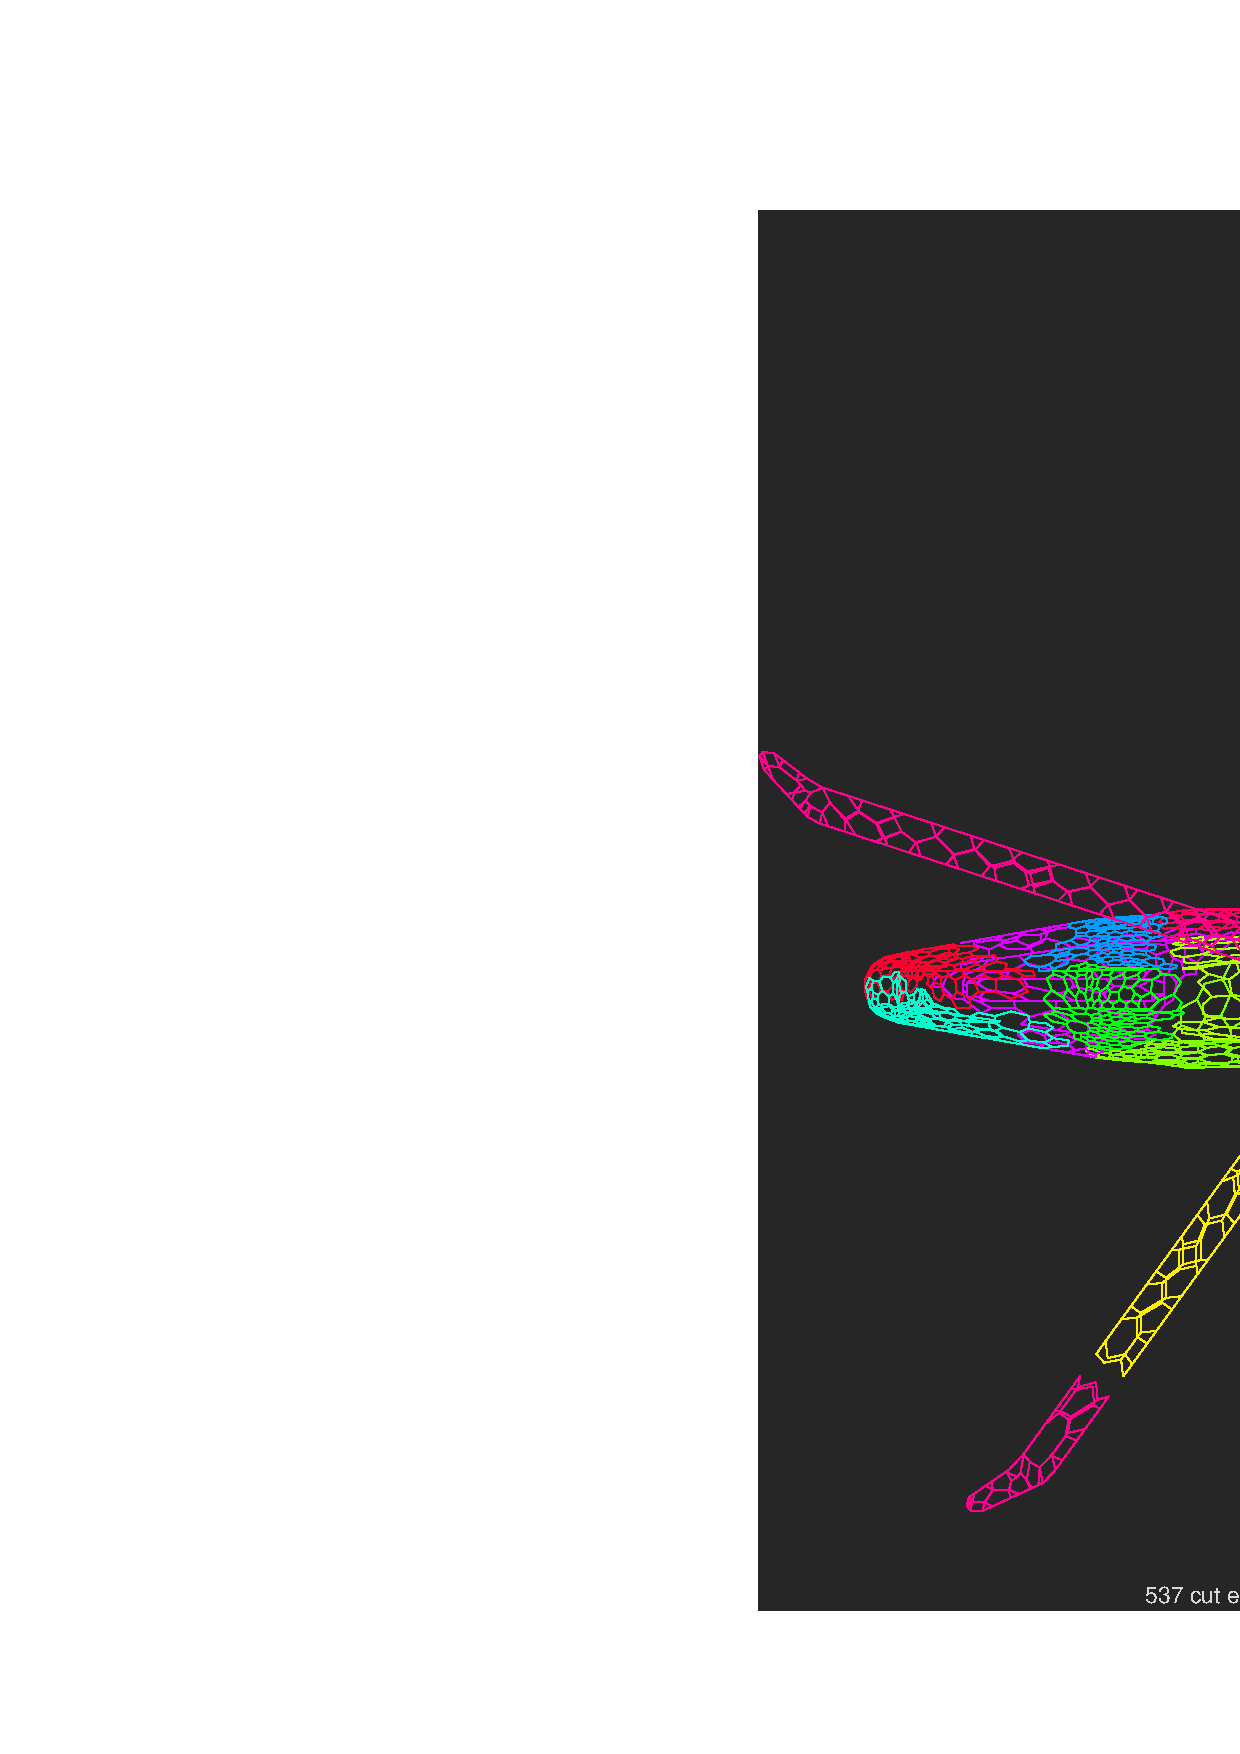
\includegraphics[width=1\textwidth, trim={0 0.5cm 0 0.5cm}, clip]{./img/ex3/heli-kway-front-32}
        \subcaption{K-way direct partitioning front view}\label{fig:heli-kway-front-32}
    \end{minipage}
    \newline
    \begin{minipage}[H]{.45\textwidth}
        \centering
        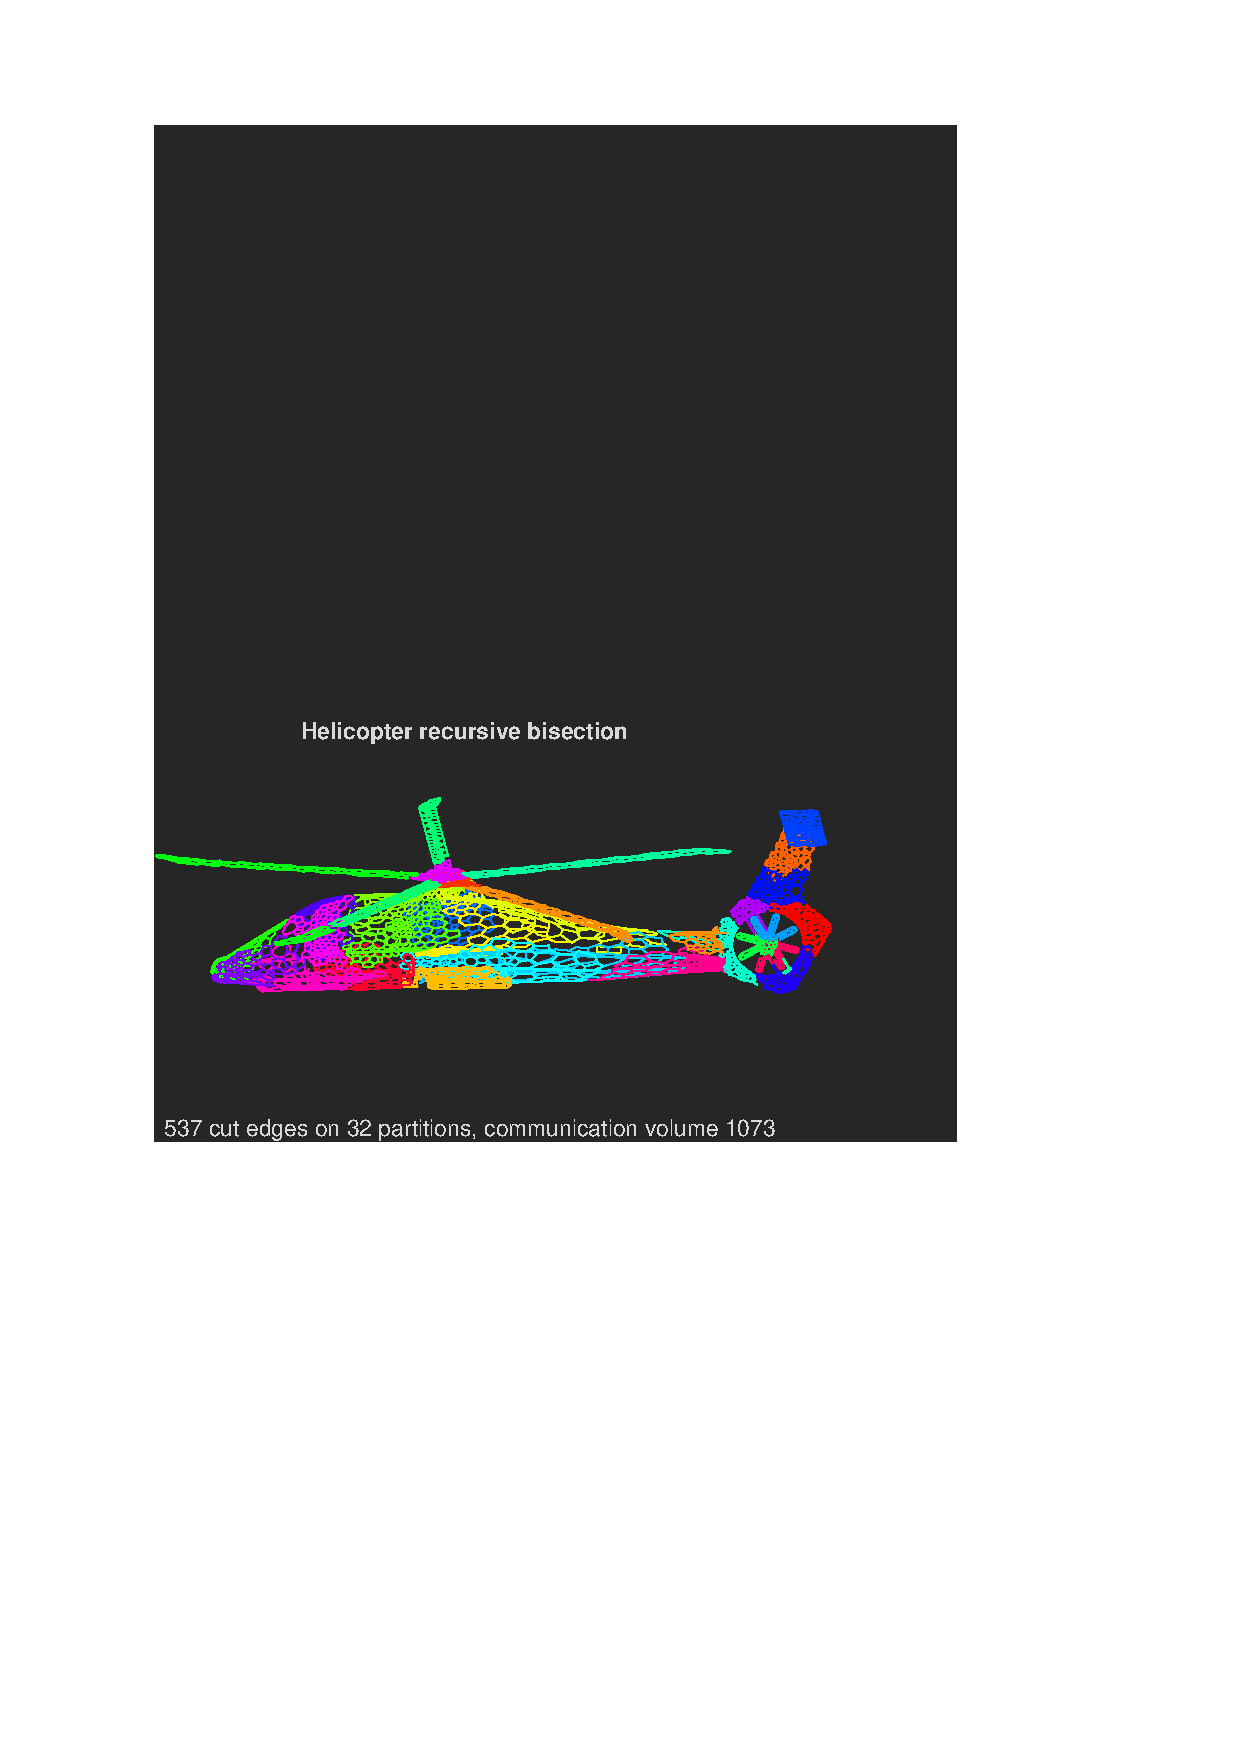
\includegraphics[width=1\textwidth, trim={0 2.1cm 0.3cm 1.2cm}, clip]{./img/ex3/heli-rec-side-32}
        \subcaption{Recursive bisection side view}\label{fig:heli-rec-side-32}
    \end{minipage}
    \hfill
    \begin{minipage}[H]{.45\textwidth}
        \centering
        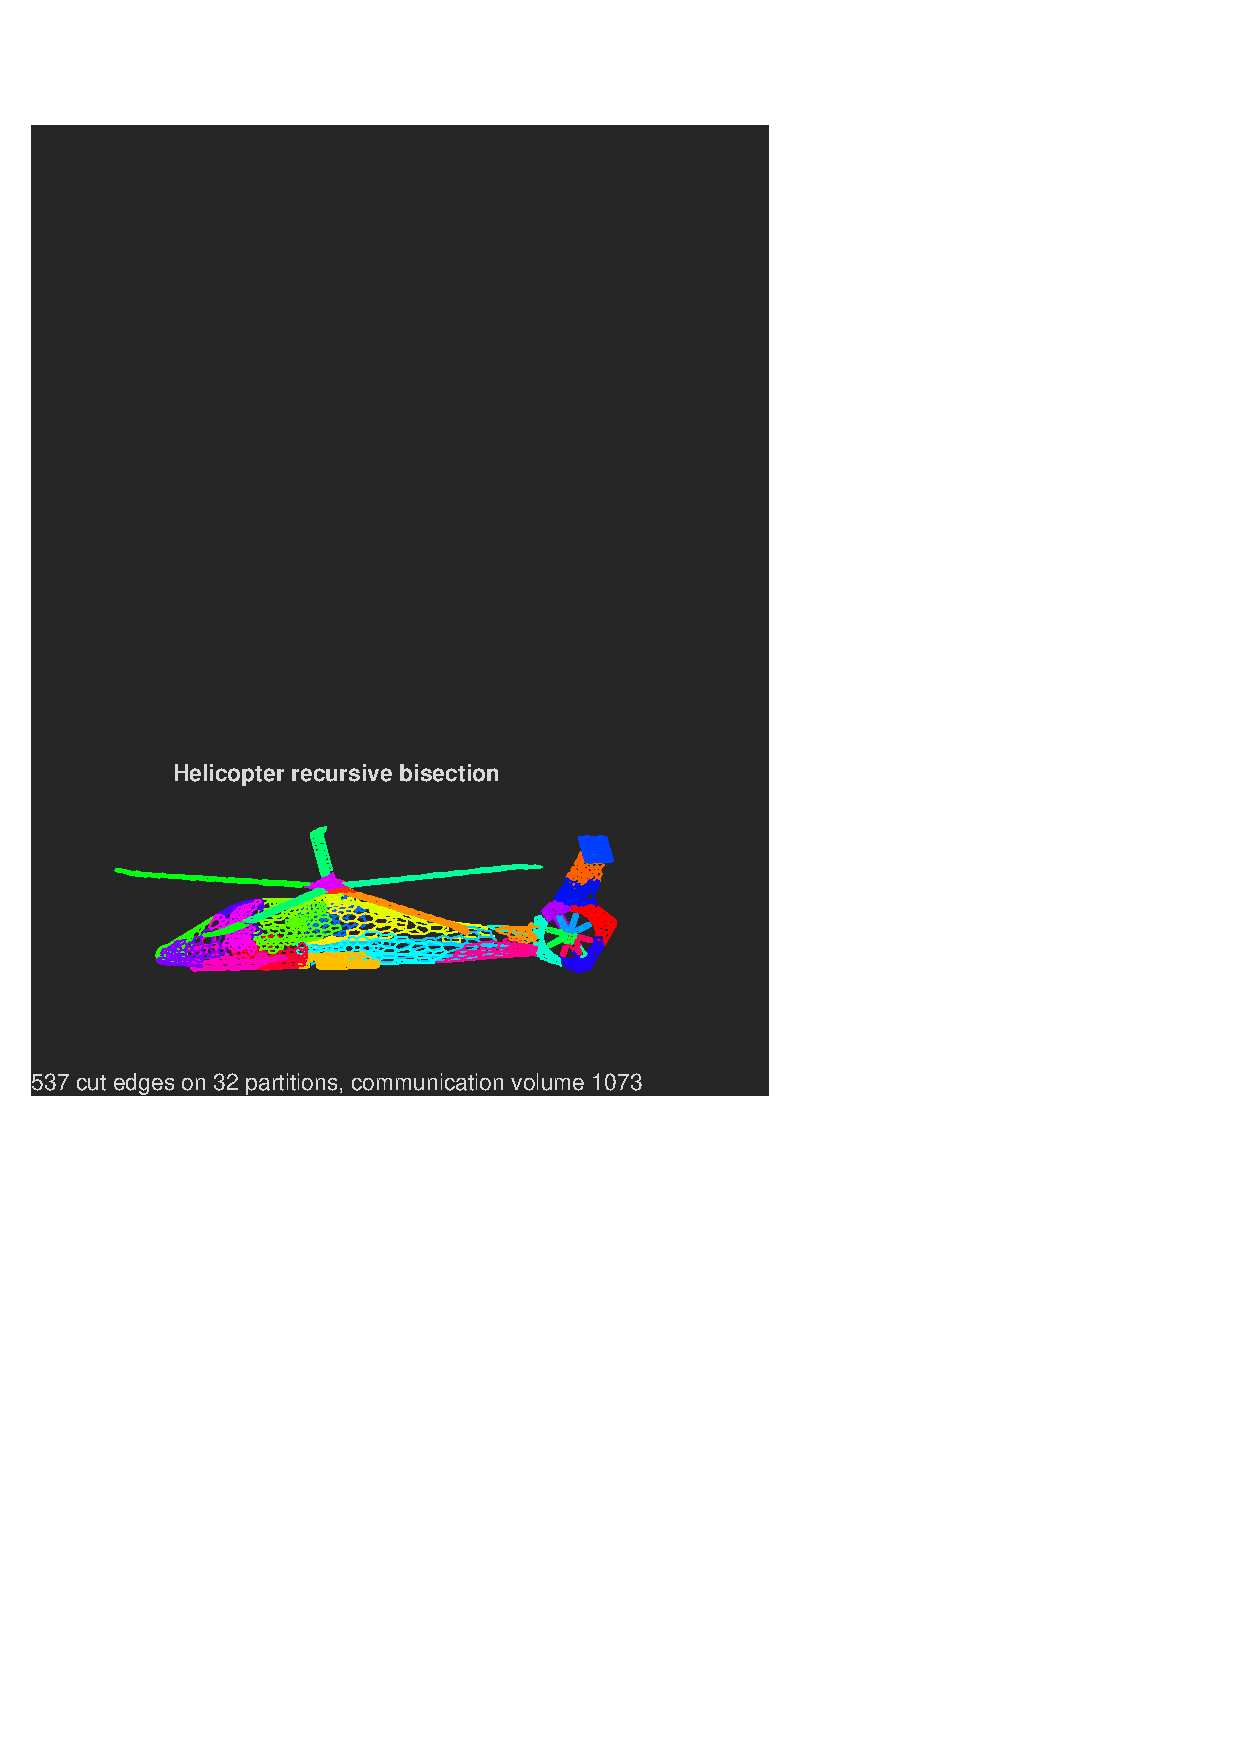
\includegraphics[width=1\textwidth, trim={1.3cm 1.8cm 1.8cm 0.9cm}, clip]{./img/ex3/heli-kway-side-32}
        \subcaption{K-way direct partitioning side view}\label{fig:heli-kway-side-32}
    \end{minipage}
    \label{fig:heli-rec-kway-32}
    \caption{\textit{commanche\_dual} mesh - method confront with $32$ partitions}
\end{figure}


\begin{figure}[H]
    \begin{minipage}[H]{.45\textwidth}
        \centering
        \includegraphics[height=\imgHeightSkirt, width=1\textwidth, trim={0.6cm 0.5cm 0.4cm 0.3cm}, clip]{./img/ex3/skirt-rec-front-32}
        \subcaption{Recursive bisection front view}\label{fig:skirt-rec-front-32}
    \end{minipage}
    \hfill
    \begin{minipage}[H]{.45\textwidth}
        \centering
        \includegraphics[height=\imgHeightSkirt, width=1\textwidth, trim={5.2cm 1.2cm 2cm 0.5cm}, clip]{./img/ex3/skirt-rec-side-32}
        \subcaption{Recursive bisection side view}\label{fig:skirt-rec-side-32}
    \end{minipage}
    \newline
    \begin{minipage}[H]{.45\textwidth}
        \centering
        \includegraphics[height=\imgHeightSkirt, width=1\textwidth, trim={0 0.5cm 0 0.35cm}, clip]{./img/ex3/skirt-kway-front-32}
        \subcaption{K-way direct partitioning front view}\label{fig:skirt-kway-front-32}
    \end{minipage}
    \hfill
    \begin{minipage}[H]{.45\textwidth}
        \centering
        \includegraphics[height=\imgHeightSkirt, width=1\textwidth, trim={5.3cm 1.2cm 1.3cm 1cm}, clip]{./img/ex3/skirt-kway-side-32}
        \subcaption{K-way direct partitioning side view}\label{fig:skirt-kway-side-32}
    \end{minipage}
    \label{fig:skirt-rec-kway-32}
    \caption{\textit{Skirt} mesh - method confront with $32$ partitions}
\end{figure}
\cleardoublepage

\subsection*{Extra: Windows 11 implementation}

Initially for the assignment, my test environment was:
\begin{itemize}
    \item Windows 11 x64 Pro Version 22H2 Build 22621.2428
    \item Matlab R2023b
    \item Metis 5.0.2
    \item CMake 3.28.0-rc2
    \item Visual Studio 17 2022 c++ compiler
\end{itemize}

Compiling process specifics are explained in this issued I commented on \href{https://github.com/dgleich/metismex/issues/2\#issuecomment-1772906999}{metismex github}.

The reason to why I didn't finish my report with such environment is that of getting different results from the ones of
my peers and TAs I talked with, and that in order to prevent any further issues I decided to switch to a Linux environment.

\subsubsection*{Implement various graph partitioning algorithms}

From table \ref{table:win-bisection}, we notice how the Metis 5.0.2 version result changes giving $4$ better results out of $6$ graphs
with respect to the precompiled GNU/Linux version provided by the professor.
Some doubts arise about the Metis version provided by the professor being really the $5.0.2$. \\

Coordinate and inertial methods remains the same while spectral implementation is worse in most cases. \\

\begin{table}[h]
    \caption{Win 11 - Bisection results}
    \centering
    \begin{tabular}{l|r|r|r|r} \hline\hline
        Mesh                       & Coordinate & Metis 5.0.2 & Spectral & Inertial \\ \hline
        grid5rec(12,100)           & 12         & 12          & 12       & 12       \\
        grid5rec(100,12)           & 12         & 14          & 12       & 12       \\
        grid5recRotate(100,12,-45) & 22         & 14          & 12       & 12       \\
        gridt(50)                  & 72         & 76          & 82       & 72       \\
        grid9(40)                  & 118        & 122         & 136      & 118      \\
        Smallmesh                  & 25         & 12          & 14       & 30       \\
        Tapir                      & 55         & 22          & 58       & 49       \\
        Eppstein                   & 42         & 41          & 47       & 45       \\
        \hline \hline
    \end{tabular}
    \label{table:win-bisection}
\end{table}

\end{document}
